% ---------------------------------------------------------------------------------------
\chapter{Experimentos Num\'ericos}\label{chap5}

    Como ya mencionamos en el cap\'itulo \ref{chap3} se utilizaron im\'agenes de la base de datos ''\textit{Kodak Lossless TrueColor Image Suite}''\ref{fig:rgb2gray_2} \cite{KodakLosslessTrueColorImageSuite}. A cada una de las correspondientes im\'agenes ser\'an pasadas a blanco y negro, como fue descrito en \ref{eq:grayscale}, y posteriormente se le aplicar\'a la transformaci\'on de Box-Cox con los tr\'es m\'etodos de selecci\'on de $\lambda$ descritos en el cap\'itulo anteror, utilizando el vector completo de la im\'agen, el histograma, y finalmente una ventana movil.

    \begin{figure}[H]
        \centering
        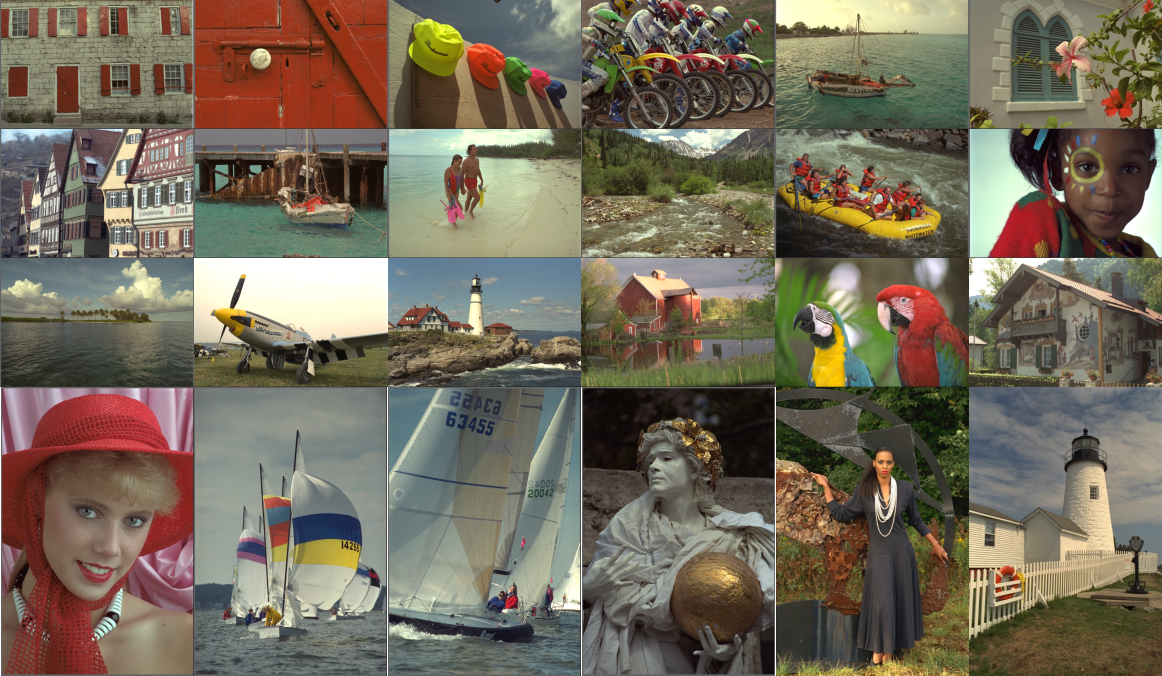
\includegraphics[width=0.8\textwidth]{all_images_grid.png}
        \caption{Banco de imagenes a utilizar.}
        \label{fig:rgb2gray_2}
    \end{figure}
    
    Ya revisamos el efecto que en general tiene cada $\lambda$ en la im\'agen de manera visual, y como la selecci\'on de este par\'ametro afecta a cada una, en la siguientes secci\'ones discutiremos la relaci\'on que existe entre una im\'agen y su transformada para $\lambda$ cualquiera en el conjunto $[-2, 5]\subset\R$ y posteriormente como se ve la relaci\'on entre una im\'agen y su transformada usando los distintos lamdba entregados por los m\'etodos ya descritos.

    A lo largo de la secci\'on usaremos las im\'agenes 1, 2, 13, y 22 del banco \cite{KodakLosslessTrueColorImageSuite}, pero los experimentos realizados para todas las imagenes pueden ser encontrados en el ap\'endice \ref{appA} del trabajo. 
    

\section[Comparando imagenes vs. lambda]{Comparando imagenes vs. $\lambda$}

    No es de interes estudiar la relaci\'on com\'un entre las im\'agnes y su transformada para un $\lambda$ cualquiera en $[-2, 5]\subset\R$. Para esto nos vamos a tomamos $31$ valores equidistantes de $\lambda$ y calculamos su correlaci\'on haciendo uso de los m\'etodos descritos en el cap\'itulo \ref{chap2}, $dCor$, $MIC$, y $\rho$ de Pearson. Notemos que para cada una de estas mediciones de correlaci\'on tenemos dos formas de aplicarlas en im\'agenes, utilizando el vector completo o utilizando el histograma de la im\'agen. 

    Ahora, veamos los resultados para algunas de las im\'agenes del banco, primero utilizando el ventor completo en la medici\'on de correlaci\'on  

    \begin{figure}[H]
        \centering
        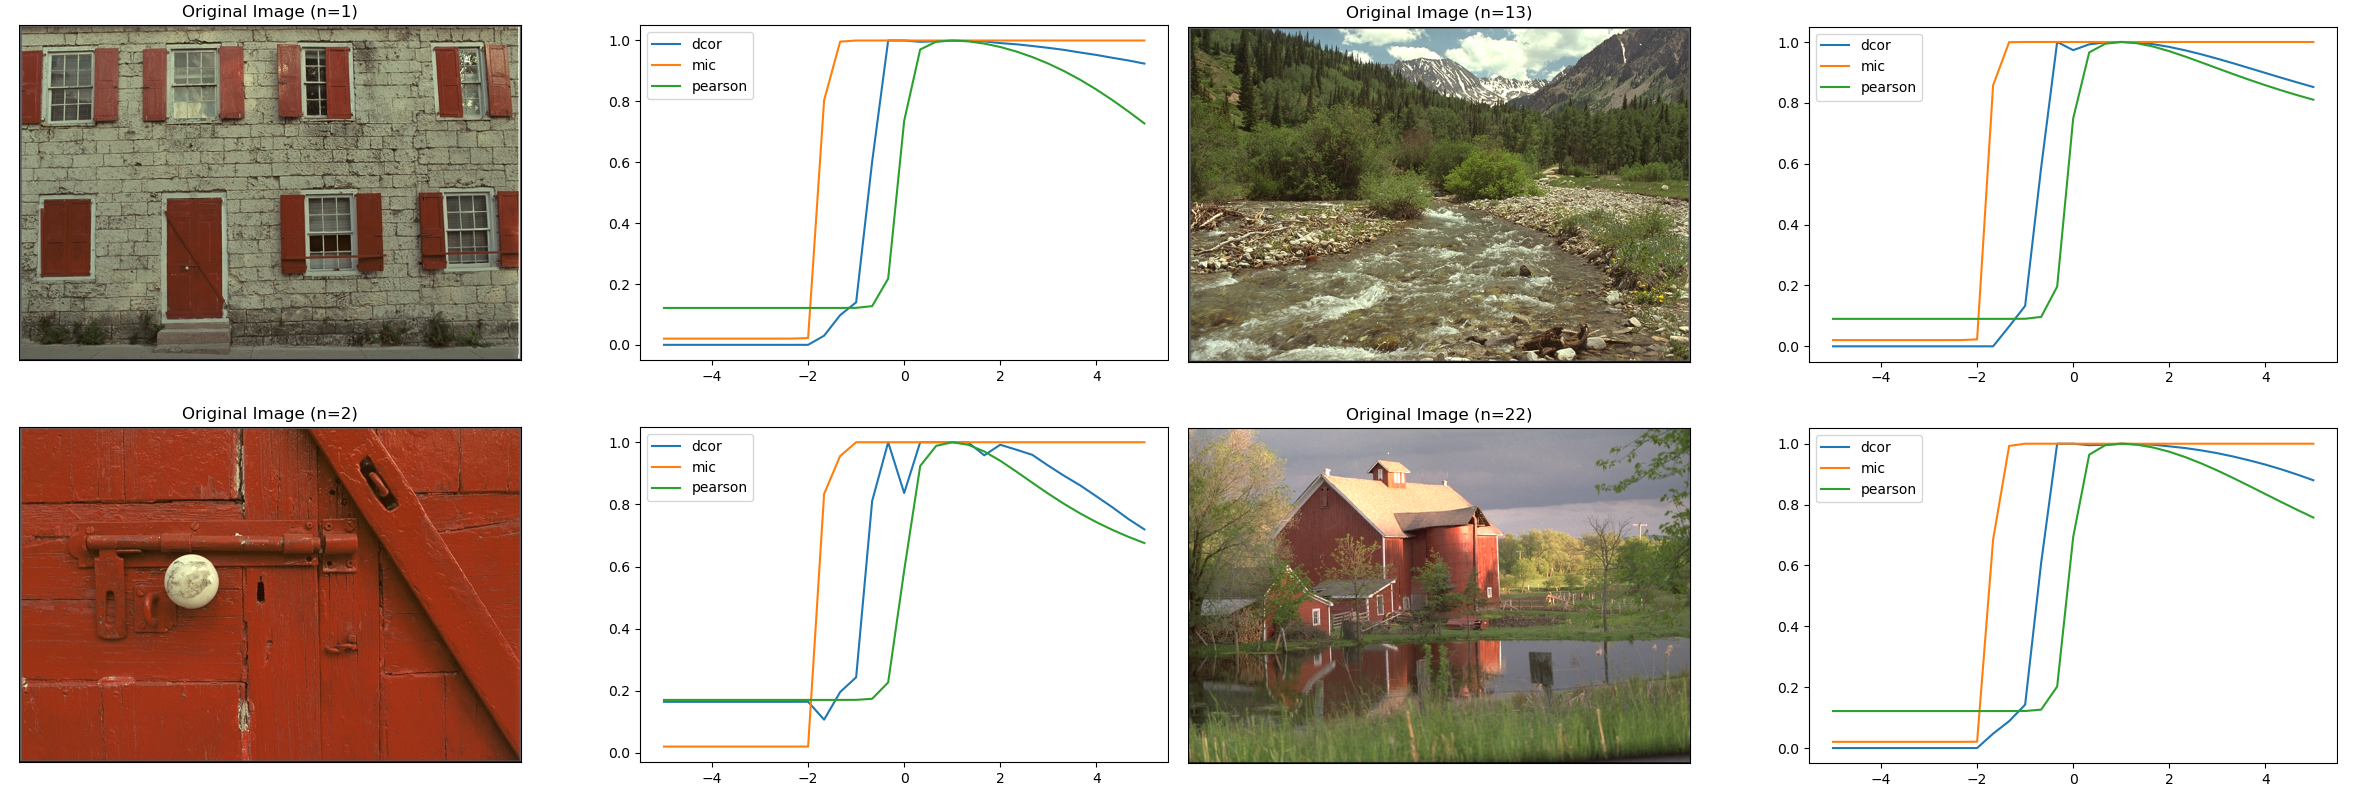
\includegraphics[width=0.7\textwidth]{lam_v_com_all_img.png}
        \caption{De arriba hacia abajo, imagenes 1, 2, 13, y 22. A la izquierda la im\'agen original y a la derecha el valor de $dCor$ (azul), $MIC$ (naranja), y $\rho$ (verde) utilizando el vector completo en el eje y, $\lambda$ en el eje x.}
    \end{figure}


    Es claro a simple vista que el comportamiento de las curvas es similar, cabe descatar que es el MIC el cual detecta la relaci\'on de forma m\'as ''temprana'', con dCor siguiendo no mucho m\'as atr\'as. Otra cosa que vale la pena mencionar es que el MIC mantiene una correlaci\'on alta con la im\'agen original, incluso para valores altos de $\lambda$, cosa que no ocurre con dCor, el cual disminuyemientas los valores de $\lambda$ van aumentando, pero de todas formas suele estar por encima de los valores de $rho$.

    Repitiendo lo anterior, pero ahora utilizando el histograma para realizar la comparaci\'on entre las im\'agenes, obtenemos:

    \begin{figure}[H]
        \centering
        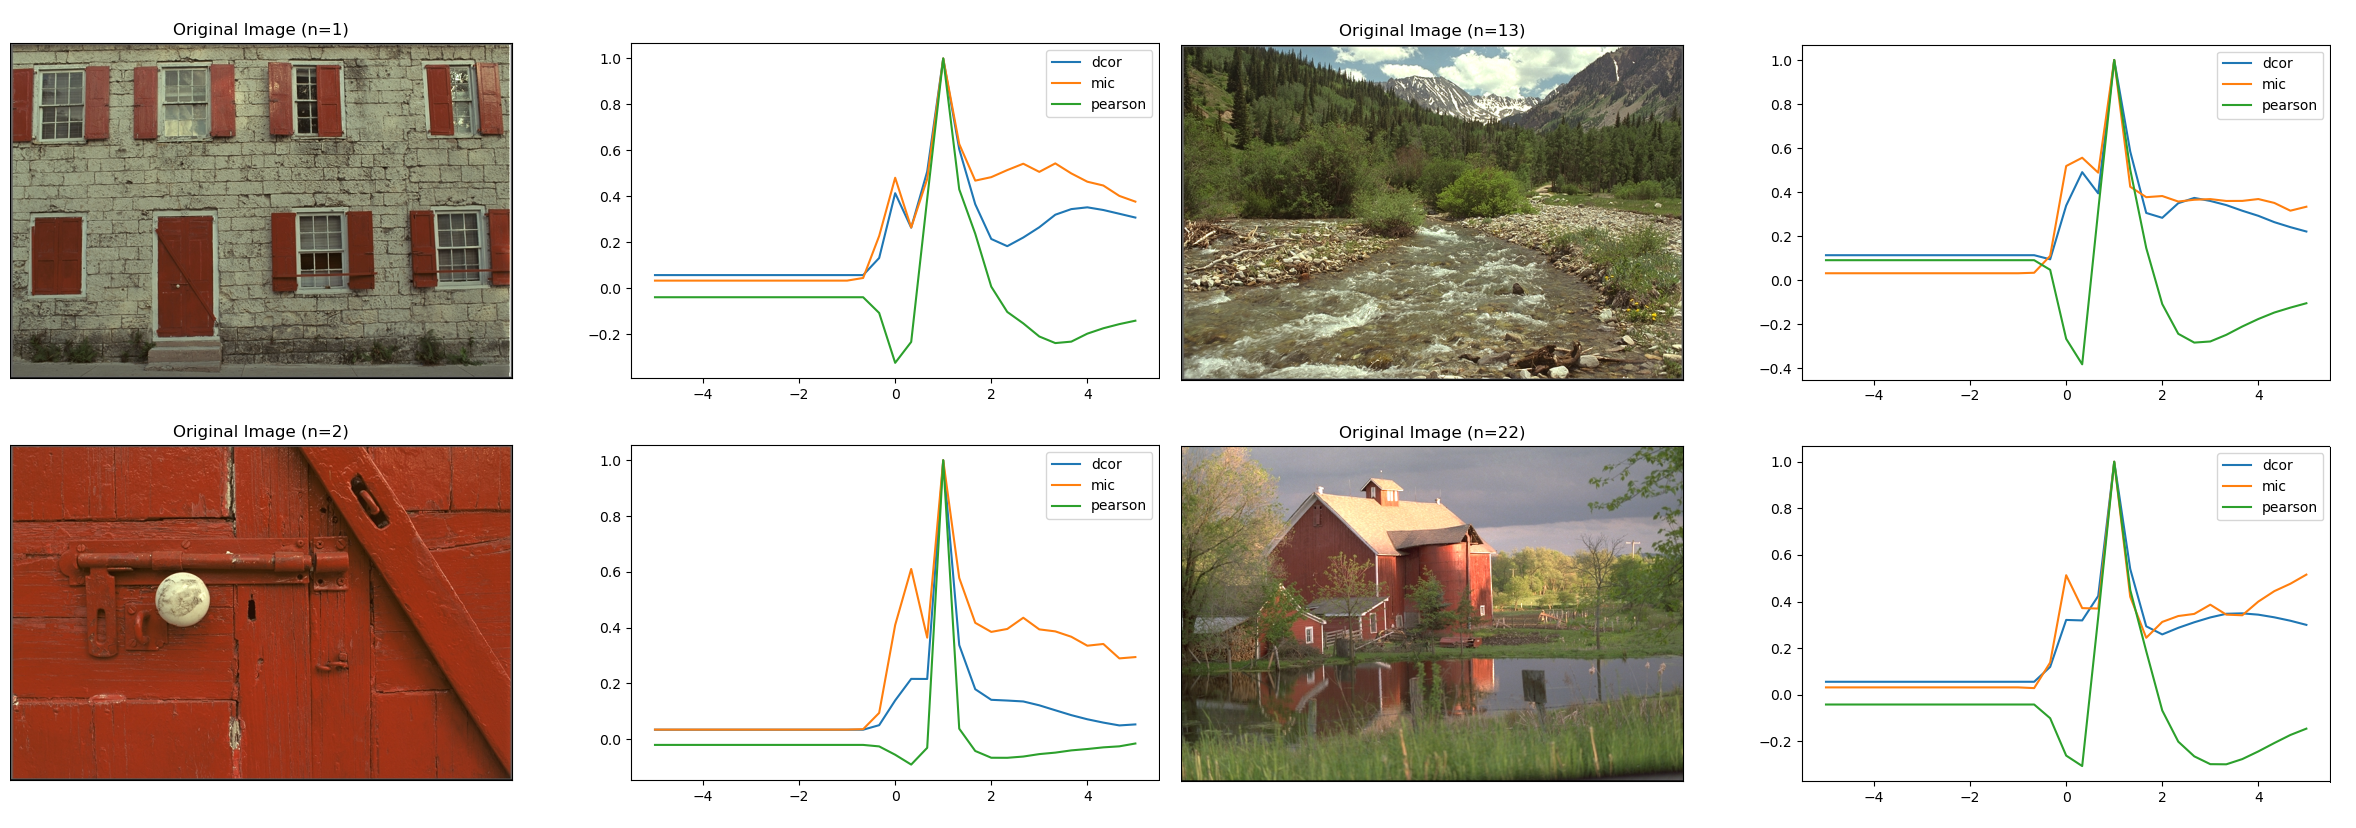
\includegraphics[width=0.7\textwidth]{lam_v_com_all_img_hist.png}
        \caption{De arriba hacia abajo, imagenes 1, 2, 13, y 22. A la izquierda la im\'agen original y a la derecha el valor de $dCor$ (azul), $MIC$ (naranja), y $\rho$ (verde) utilizando el histograma en el eje y, $\lambda$ en el eje x.}
    \end{figure}

        Podemos notar un comportamiento similar entre estos resultados y los mostrados al usar el vector de la im\'agen de forma completa, pero en general con valores m\'as d\'ebiles. De la misma forma tambi\'en es el $MIC$ es cu\'al es capaz de identificar la relaci\'on de forma m\'as ''temprana'', adem\'as de que nuevamente este se encuentra por encima de $dCor$ en casi todo momento.

        Otra cosa destacable y en donde se distancian estos resultados de los anteriores, es en la aparici\'on de valores negativos de $\rho$ para algunos valores de $\lambda$. 

        Esto en general nos indica que desde cierto valor de $\lambda$, en este caso $-2$ al momentod de comprar vectores completos, y $-0.5$ para la comparaci\'on de los histogramas, existe una fuerte correlaci\'on entre la im\'agen y el resultado de la trnaformaci\'on Box-Cox, esto se ve principalmente reflejado en el alto valor que los tres valores de comparaci\'on al usar la im\'agen completa, y en los valores relativamente altos al realizar la comparacion con los histogramas. 

        Por \'ultimo vale la pena mencionar que, al menos al momento de comparar los histogramas de las im\'agenes, $rho$ no nos entrega buenos resultados. 


\section{Comparando imagenes con su tranformada}

    Ya habiendo revisado la relaci\'on que tienen las im\'agenes dado un rango de valores para $\lambda$, ahora nos enfocamos en revisar los valores de correlaci\'on para los $\lambda$'s obtenidos utilziando los m\'etodos descritos en el cap\'itulo \ref{chap4}. 
    
    De la misma forma que en la secci\'on anterior, comenzaremos analizando los valores de $dCor$, $MIC$, y $rho$, para cada im\'agen.
    
    \begin{figure}[H]
        \centering
        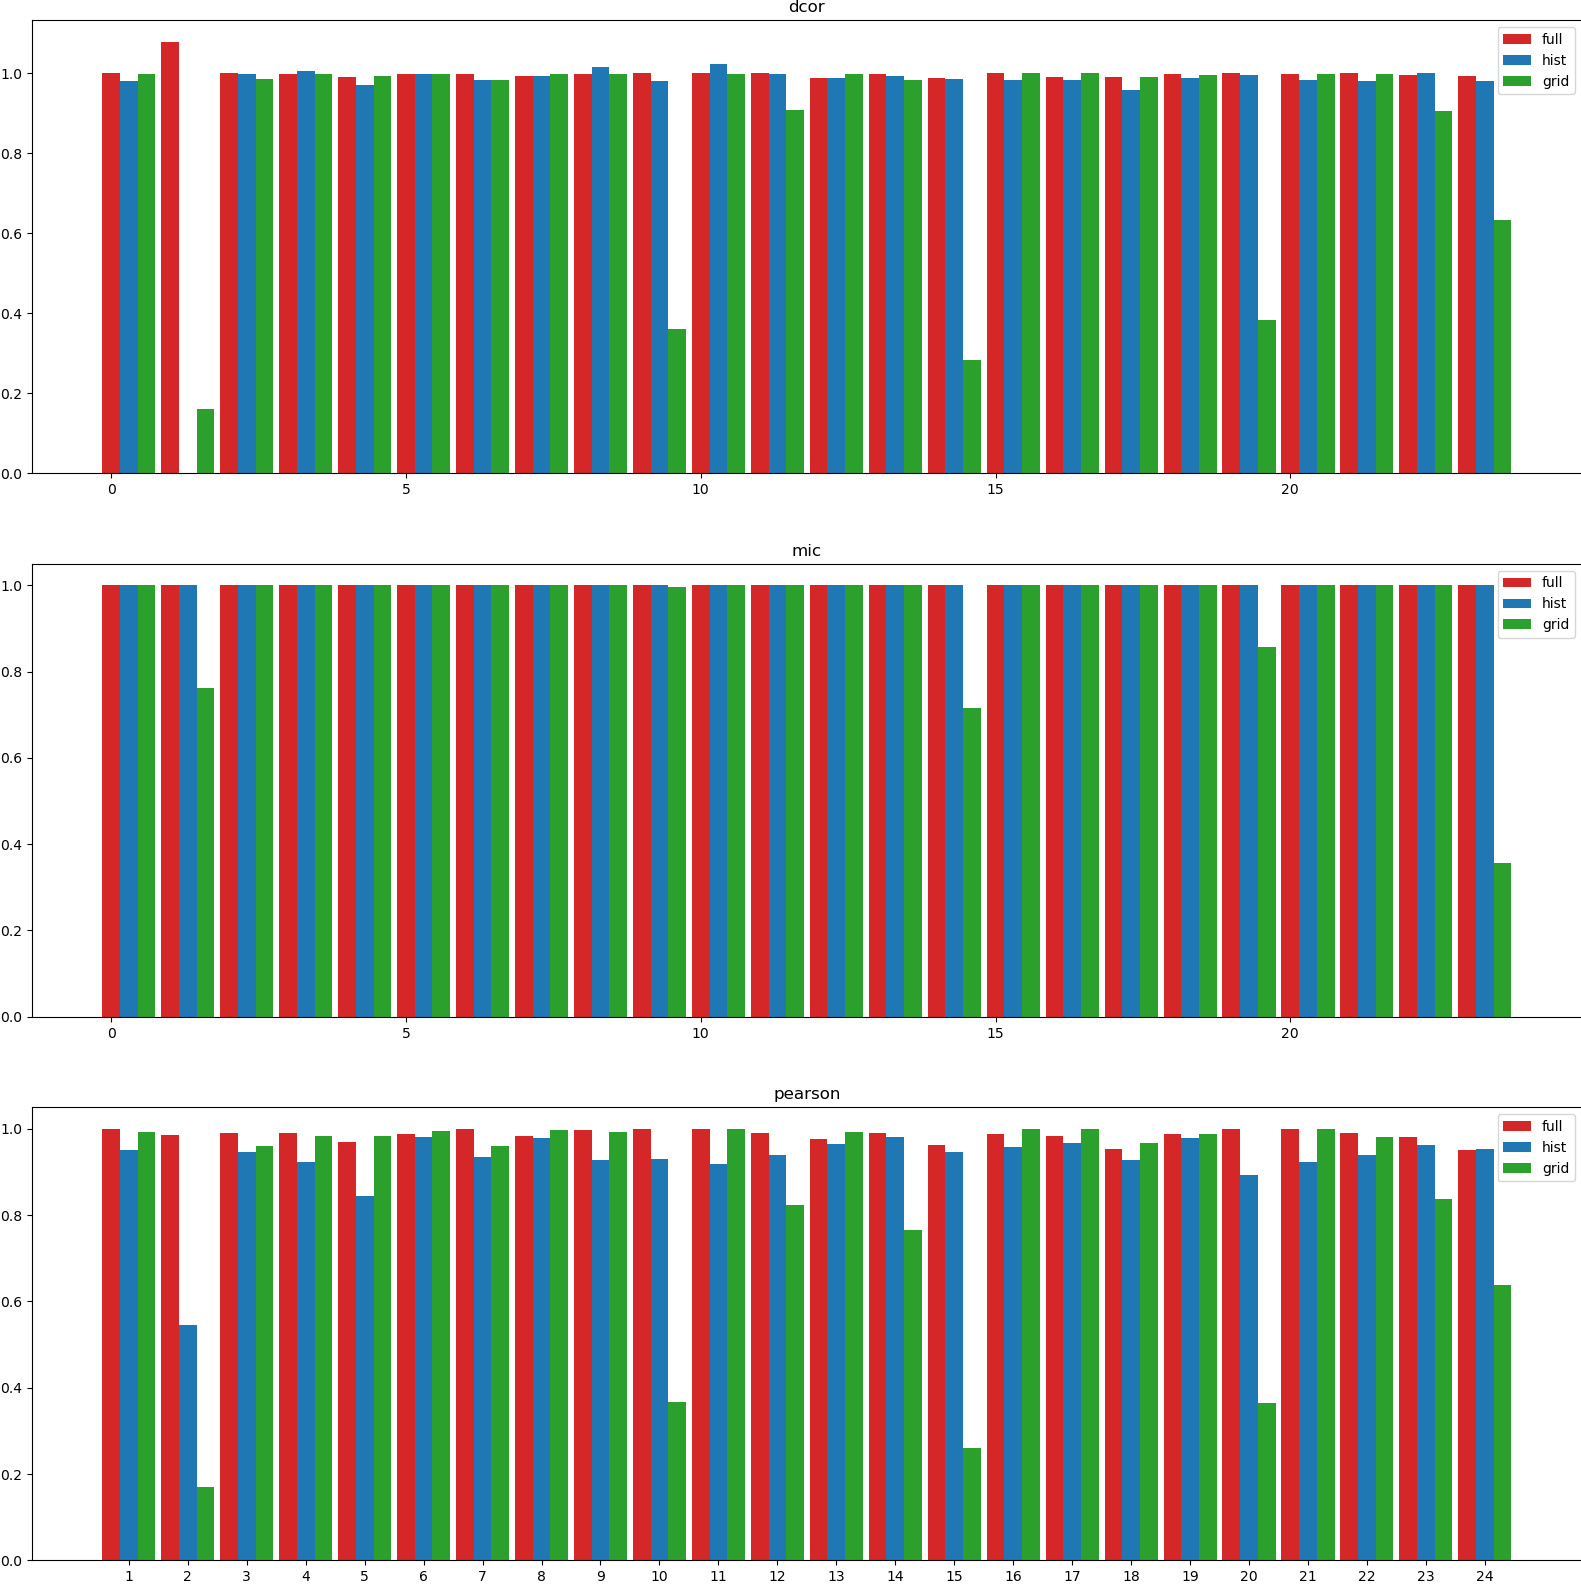
\includegraphics[width=0.7\textwidth]{plot_comparison_full.png}
        \caption{Valores de dcor, mic y pearson para cada imagen usando todo el vector, azul es el metodo para encontrar $\lambda$ con toda la imagen, rojo es el histograma y verde es el grid}
    \end{figure}

    Como era de esperar por lo que vimos en la secci\'on anterior, los valores de las correlaciones utilizando todo el vector son bastante altas, siendo los valores de $\rho$ ligeramente m\'as pequen\~os que el resto. 

    Otra cosa que vale la pena mencionar son los valores ''an\'omalos'' que ocurren para el m\'etodo de grilla, en particular para las im\'agenes 2, 10, 15, y 20. Para explicar esto veamos las im\'agenes en cuestion

    \begin{figure}[H]
        \centering
        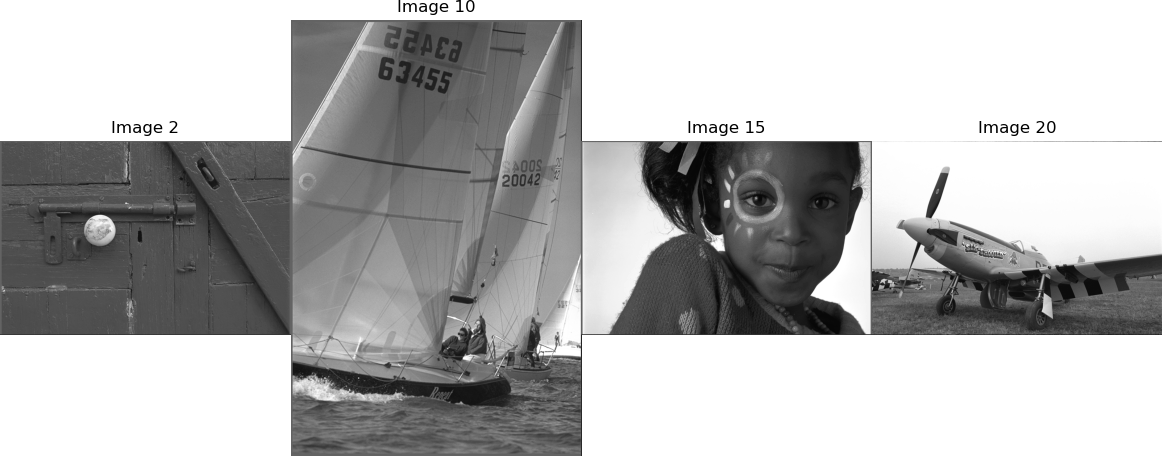
\includegraphics[width=0.75\textwidth]{anomalies_grid.png}
        \caption{De izquierda a derecha, im\'agenes 2, 10, 15, 20, y 24 del bamco \cite{KodakLosslessTrueColorImageSuite}}
    \end{figure}

    Podemos ver que estas im\'agenes sufren del mismo problema descrito en el cap\'itulo \ref{chap4}, donde imagenes con grandes secciones de similar color generan problemas al momento de calcular un $\lambda$.

    Antes de revisar los valores haciendo uso de los histogramas, revisemos los promedios de las comparaciones. 

    \begin{table}[H]
        \centering
        \begin{tabular}{|l|l|l|}
            \hline
        Correlaci\'on    & $\lambda$ & Valor  \\    \hline
        dcor    & Completo    & 1.000  \\
        mic     & Completo    & 1.000  \\
        mic     & Histograma  & 1.000  \\
        pearson & Completo    & 0.985 \\
        dcor    & Histograma  & 0.948 \\
        mic     & Grilla      & 0.945  \\
        pearson & Histograma  & 0.925  \\
        dcor    & Grilla      & 0.856  \\
        pearson & Grilla      & 0.945  \\     \hline

        \end{tabular}
    \end{table}

    Ya con esto es claro ver que los valores m\'as altos fueron alcanzados por el m\'etodo de selecci\'on de  $\lambda$ que utiliza todo el vector de datos es el cual m\'antiene posee la mayor correlaci\'on, seguido por el histograma y finalmente el m\'etodo de grilla. Otra cosa que podemos destacar es que pearson present\'o los valores m\'as bajos en general.

    Veamos ahora como se ve la situaci\'on al realizar la comparaci\'on haciendo uso de los histogramas.

    \begin{figure}[H]
        \centering
        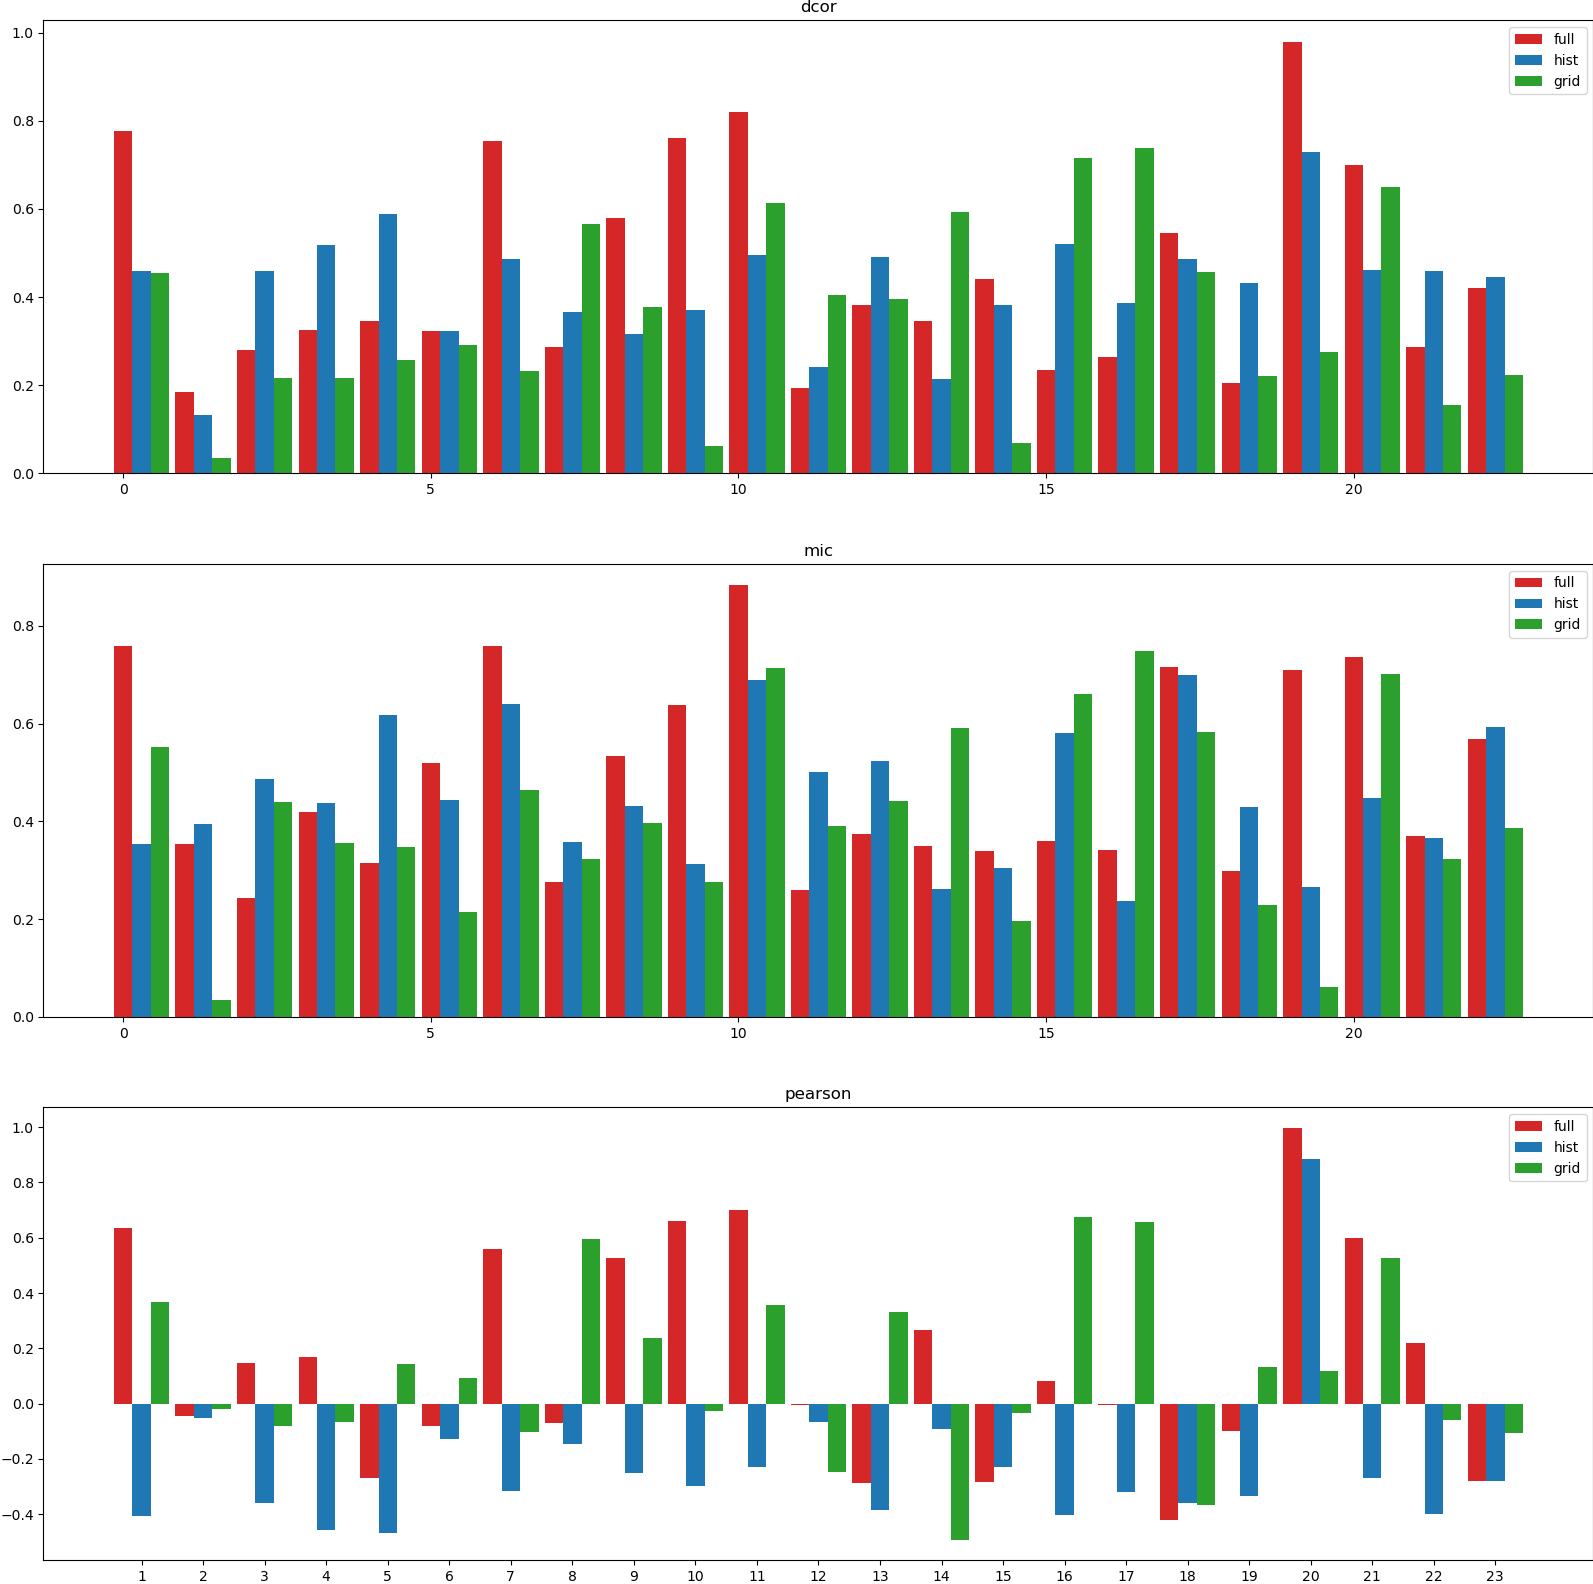
\includegraphics[width=0.7\textwidth]{plot_comparison_hist.png}
        \caption{Valores de dcor, mic y pearson para cada imagen usando el histograma, azul es el metodo para encontrar $\lambda$ con toda la imagen, rojo es el histograma y verde es el grid}
    \end{figure}

    Esto ya nos entrega resultaos un poco m\'as complejos, pero de todas formas hay algunas tendencias claras. Pero antes de concluir revisemos los promedios de estas variables.

    \begin{table}[H]
        \centering
        \begin{tabular}{|l|l|l|}\hline
        mic     & Completo    & 0.487  \\\hline
        dcor    & Completo    & 0.459  \\
        mic     & Histograma  & 0.457  \\
        dcor    & Histograma  & 0.431  \\
        mic     & Grilla      & 0.398  \\
        dcor    & Grilla      & 0.346 \\
        pearson & Completo    & 0.108  \\
        pearson & Grilla      & 0.108  \\
        pearson & Histograma  & -0.225 \\\hline
        \end{tabular}
    \end{table}
    
    De las misma forma que en el an\'alisis anterior, podemos ver que el m\'etodo completo fue el que mantuvo el mayor valor de correlaci\'on, seguido por el histigrama y finalmente la grilla. 
    
    Confirmamos adem\'as algo que parecia ser claro en base a los gr\'aficos, el $MIC$ se encuentra, por lo general, por encima del $dCor$, cosa que es corroborada por el hecho de que el valor del promdeio del $MIC$, es siempre mayor que el de $dCor$ para un m\'etodo de selecci\'on de $\lambda$ dado.